\documentclass[10pt,dvipdfmx]{jsarticle}
\usepackage{ascmac}
\usepackage[margin=15truemm]{geometry}
\usepackage{amsmath}
\usepackage[dvipdfmx]{graphicx}
\setlength{\columnseprule}{0.3mm}


\begin{document}

\title{信号処理特論 第9回課題}
\author{視覚認知システム研究室\\学籍番号:2433730032 岡村 翼}
\date{\today}
\maketitle

{\textgt{課題} }
課題1より、πを求めなさい。
横軸 n 、縦軸を4k/nとして、4k/nがπに漸近することを確かめる。\\

0から1の範囲の独立変数を乱数で2つ生成し、モンテカルロ法により$\pi$の近似値を求めた。\\
$(n,4k/n)$のグラフを図1に示す。\\
  \begin{figure}[h]
    \begin{center}
      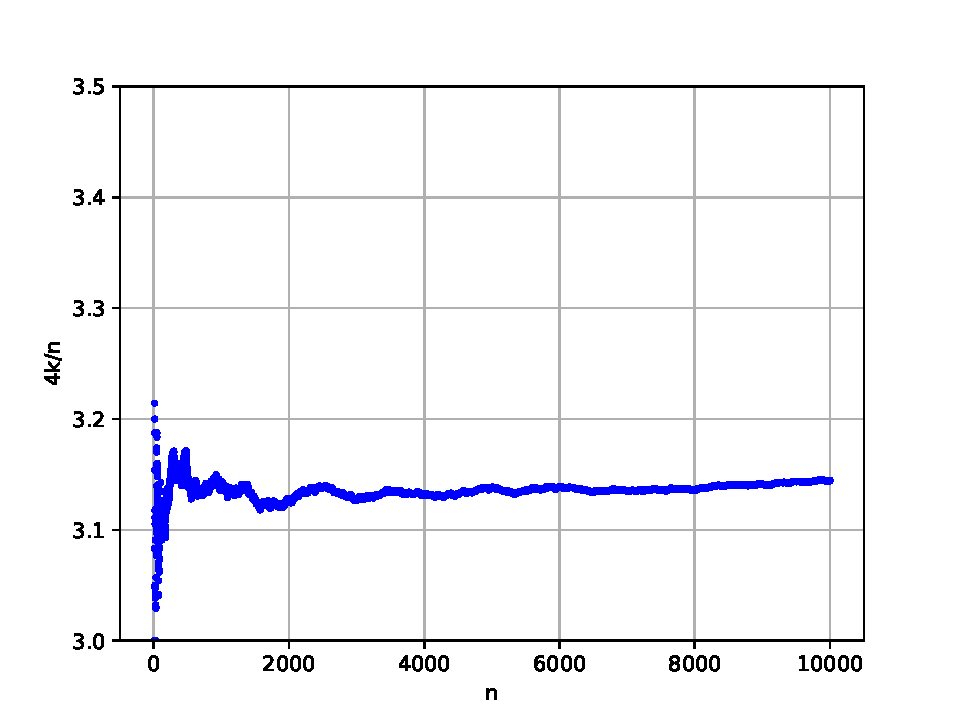
\includegraphics{Montecarlo.pdf}
      \caption{モンテカルロ法}
      \label{1}
    \end{center}
  \end{figure}
グラフより、$4k/n$が$\pi$に漸近することが確かめられた。\\
(なお、pythonによって計算を行い、乱数の生成にはrandomモジュールのrandom.random()を使用した。)
\end{document}